\documentclass[a4paper,landscape]{article}

%% Required to make the text fill the page better
\usepackage[textwidth=20cm]{geometry}

% Required for specifying captions to tables and figures
\usepackage[font=small,labelfont=bf]{caption}

%% Required to display some mathematical formula
\usepackage{amsmath,amssymb}

%% So that I can draw the graphs for the confidence in difference
\usepackage{tkz-graph}
\renewcommand*{\EdgeLineWidth}{0.15pt}

%% So that I can display the plots
\usepackage{graphicx}

%% Sets the font family for the document to a sans-serif font
\renewcommand{\familydefault}{\sfdefault}


%% pdflatex hw2_tchlux.tex && evince hw2_tchlux.pdf 

\begin{document}

\subsection*{\hfil Comparing Throughput CDF's of 3 System Configurations \hfil}
\begin{center}
  March $22^{nd}$, 2017\\
  Thomas Lux
\end{center}

\subsection*{Summary}

In this report, we compare the Cumulative Distribution Functions
(CDF's) of the Throughput of three different system
configurations. All three configurations have the same settings for:
\begin{align*}
  Frequency  &-  2700000\\
  Hyp\ Sched &-  CFQ\\
  VM\ Sched  &-  NOOP\\
  Threads    &-  64\\
  Mode       &-  Fread
\end{align*}

While the file and record sizes for the three system settings were:
\begin{align}
  File\ Size - 64  \ \  &\ \ Record\ Size - 32\\
  File\ Size - 1024\ \  &\ \ Record\ Size - 32\\
  File\ Size - 1024\ \  &\ \ Record\ Size - 512
\end{align}

Most notably, from this in-depth comparison, it appears that our
independently drawn samples from the systems are not always conforming
to the same underlying distribution. If this trend continues, then it
will prohibit the effective modelling goals of the VarSys project.

\subsection*{Source Data}

For each of these system configurations we have 3 independently
gathered sets of data:
\begin{itemize}
\item The \textit{First} \textbf{40} runs collected for the VarSys data mid-last
  year.
\item The \textit{Second} set of \textbf{40} runs collected December of last year.
\item The newest, \textit{True} set of \textbf{420} runs collected two weeks ago.
\end{itemize}

\pagebreak
\subsection*{Figures and Plots}

For each of the three system configurations, there is 1 figure
followed by 3 plots:
\begin{enumerate}
\item The \textbf{Paired KS Solved for Alpha Graph} shows the trials
  \textit{first}, \textit{second}, and \textit{true} as nodes with the
  edges between them being the result of solving the KS Two Sample
  test for alpha (see explanation in item 4 below). This will be
  followed by the 'Confidence' interpretation below.

\item The \textbf{CDF Comparison Plot} shows the Throughput CDF's of
  each of the \textit{first}, \textit{second}, and \textit{true} data
  sets. Each CDF plot also has a red-tinted cloud~\footnote{The clouds
    were generated by taking 10,000 random 40 sample subsets of the
    (\textit{true}) 420, calculating the CDF's of each subset, then
    calculating the percentiles of possible \textit{true} CDF values
    based on the sapmle CDF's.} of the possible positions that the
  \textit{true} CDF could take on when collecting 40 sample subsets.

\item The \textbf{Kolmogorov-Smirnov (KS) Difference Plot} shows the
  decrease in KS difference~\footnote{The two-sample KS Difference is
    simply the maximum difference between the two CDF's of the
    samples. From this difference, a test is performed to determine if
    the two distributions are different.}  between a subsapmle and the
  \textit{true} CDF with increasing subsample size (x-axis).

\item The \textbf{Confidence in KS Difference Plot} shows what happens
  when we take the typical KS test for difference:
  \begin{align*}
    \text{KS Diff} &> c(\alpha) \sqrt{\frac{n_1 + n_2}{n_1 \cdot n_2}}\\
    \text{where}\ c(\alpha) &= \sqrt{-\frac{1}{2}ln\bigg(\frac{\alpha}{2}\bigg)}
  \end{align*}
  and use our knowledge of $n_1$, $n_2$ and the KS Difference to solve
  for the minimum alpha such that this inequality holds. Giving us:
  \begin{align*}
    \alpha\ \  >\ \  2 \cdot e^{-2 \cdot \bigg(\frac{\text{KS Diff}}{\sqrt{\frac{n_1 + n_2}{n_1 \cdot n_2}}}\bigg)^2}
  \end{align*}
  This final plot shows $100 \cdot (1 - \alpha)$, or the approximate
  confidence, in percentage, that the two distributions being compared
  are different. This data was collected by comparing the CDF's of 100
  random subsamples of size $\textless$x-axis$\textgreater$ to the
  \textit{true} CDF. The corresponding y-values are displayed in shaded
  regions by percentile.Ideally we want this quantity to go to zero.

\end{enumerate}

%% \textbf{Commentary:}\\
%% Notice that something.

\pagebreak
\vspace*{0.5cm}
\subsection*{\hfil System Setting \#1: File Size 64 and Record Size 32 \hfil}
\vspace*{1.0cm}

\begin{center}
  Paired KS Solved for Alpha: \\
  \vspace{0.5cm}

  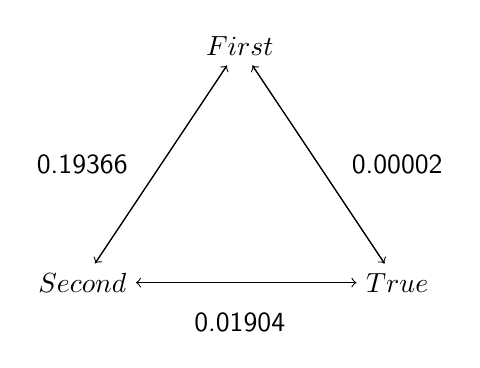
\begin{tikzpicture}
    \GraphInit[vstyle=Empty]
    %% Draw the nodes
    \node (A) at (5,3) {$First$};
    \node (B) at (3,0) {$Second$};
    \node (C) at (7,0) {$True$};
    %% Draw the alpha values
    \node (AB) at (3,1.5) {0.19366};
    \node (AC) at (7,1.5) {0.00002};
    \node (BC) at (5,-.5) {0.01904};
    %% Draw the edges
    \begin{scope}[every path/.style={->}]
      \draw (A) -- (B);
      \draw (B) -- (A);
      \draw (A) -- (C);
      \draw (C) -- (A);
      \draw (B) -- (C);
      \draw (C) -- (B);
    \end{scope}
  \end{tikzpicture}

  \vspace{1cm}
  Translated to confidence in paired difference: \\
  \vspace{0.5cm}

  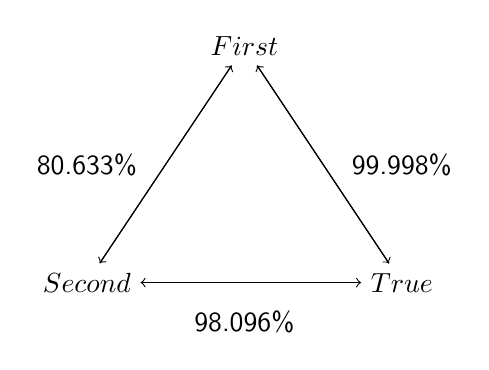
\begin{tikzpicture}
    \GraphInit[vstyle=Empty]
    %% Draw the nodes
    \node (A) at (5,3) {$First$};
    \node (B) at (3,0) {$Second$};
    \node (C) at (7,0) {$True$};
    %% Draw the alpha values
    \node (AB) at (3,1.5) {80.633\%};
    \node (AC) at (7,1.5) {99.998\%};
    \node (BC) at (5,-.5) {98.096\%};
    %% Draw the edges
    \begin{scope}[every path/.style={->}]
      \draw (A) -- (B);
      \draw (B) -- (A);
      \draw (A) -- (C);
      \draw (C) -- (A);
      \draw (B) -- (C);
      \draw (C) -- (B);
    \end{scope}
  \end{tikzpicture}
\end{center}


\vspace*{-3.5cm}
\hspace*{-3.5cm}
\includegraphics[page=1,width=27cm]{Raw-and-Fit-Report-Convergence-Over-100-Trials}
\captionof{figure}{In this CDF comparison, the \textit{first} CDF
  exceeds the reasonable bounds of \textit{true} the most, followed
  closely by \textit{second}.}

\vspace*{-3.5cm}
\hspace*{-3.5cm}
\includegraphics[page=2,width=27cm]{Raw-and-Fit-Report-Convergence-Over-100-Trials}
\captionof{figure}{In this KS Difference Plot, notice that most of the
  convergence happens with approximately 30 samples from the true
  distribution. \\This trend is common across all three system settings.}

\vspace*{-3.5cm}
\hspace*{-3.5cm}
\includegraphics[page=3,width=27cm]{Raw-and-Fit-Report-Convergence-Over-100-Trials}
\captionof{figure}{In this Confidence in KS Difference plot notice
  that we do not guarantee large improvements in confidence even with
  hundreds of samples from the distribution. This may seem to
  contradict the decreasing KS difference as seen in \textit{figure 2},
  but the slower decrease in confidence is due to the fact that the
  KS-difference test becomes more strict with increasingnly large
  sample sizes.}


%================================
%     Begin System Setting 2     
%================================

\pagebreak
\vspace*{0.5cm}
\subsection*{\hfil System Setting \#2: File Size 1024 and Record Size 32 \hfil}
\vspace*{1cm}


\begin{center}
  Paired KS Solved for Alpha:\\
  \vspace{0.5cm}  

  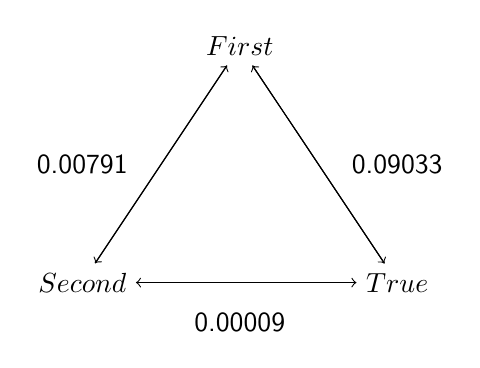
\begin{tikzpicture}
    \GraphInit[vstyle=Empty]
    %% Draw the nodes
    \node (A) at (5,3) {$First$};
    \node (B) at (3,0) {$Second$};
    \node (C) at (7,0) {$True$};
    %% Draw the alpha values
    \node (AB) at (3,1.5) {0.00791};
    \node (AC) at (7,1.5) {0.09033};
    \node (BC) at (5,-.5) {0.00009};
    %% Draw the edges
    \begin{scope}[every path/.style={->}]
      \draw (A) -- (B);
      \draw (B) -- (A);
      \draw (A) -- (C);
      \draw (C) -- (A);
      \draw (B) -- (C);
      \draw (C) -- (B);
    \end{scope}
  \end{tikzpicture}

  \vspace{1cm}
  Translated to confidence in paired difference: \\
  \vspace{0.5cm}

  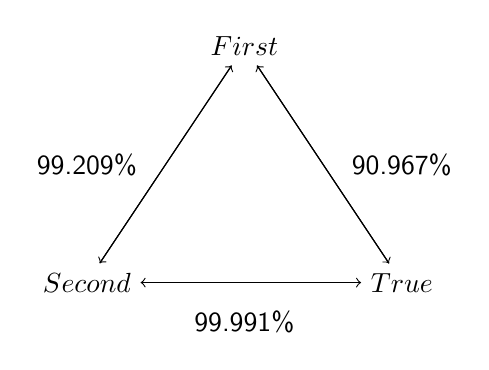
\begin{tikzpicture}
    \GraphInit[vstyle=Empty]
    %% Draw the nodes
    \node (A) at (5,3) {$First$};
    \node (B) at (3,0) {$Second$};
    \node (C) at (7,0) {$True$};
    %% Draw the alpha values
    \node (AB) at (3,1.5) {99.209\%};
    \node (AC) at (7,1.5) {90.967\%};
    \node (BC) at (5,-.5) {99.991\%};
    %% Draw the edges
    \begin{scope}[every path/.style={->}]
      \draw (A) -- (B);
      \draw (B) -- (A);
      \draw (A) -- (C);
      \draw (C) -- (A);
      \draw (B) -- (C);
      \draw (C) -- (B);
    \end{scope}
  \end{tikzpicture}
\end{center}

\vspace*{-3.5cm}
\hspace*{-3.5cm}
\includegraphics[page=4,width=27cm]{Raw-and-Fit-Report-Convergence-Over-100-Trials}
\captionof{figure}{In this CDF comparison, the \textit{second} CDF is
  most notably an outlier. This is reflected in the solved alpha graph
  above.}

\vspace*{-3.5cm}
\hspace*{-3.5cm}
\includegraphics[page=5,width=27cm]{Raw-and-Fit-Report-Convergence-Over-100-Trials}
\captionof{figure}{This KS Difference Plot follows similar trends to
  the previous.}

\vspace*{-3.5cm}
\hspace*{-3.5cm}
\includegraphics[page=6,width=27cm]{Raw-and-Fit-Report-Convergence-Over-100-Trials}
\captionof{figure}{This Confidence in KS Difference plot follows
  similar trends to the previous.}


%================================
%     Begin System Setting 3     
%================================

\pagebreak
\vspace*{0.5cm}
\subsection*{\hfil System Setting \#3: File Size 1024 and Record Size 512 \hfil}
\vspace*{1cm}

\begin{center}
  Paired KS Solved for Alpha:\\
  \vspace{0.5cm}

  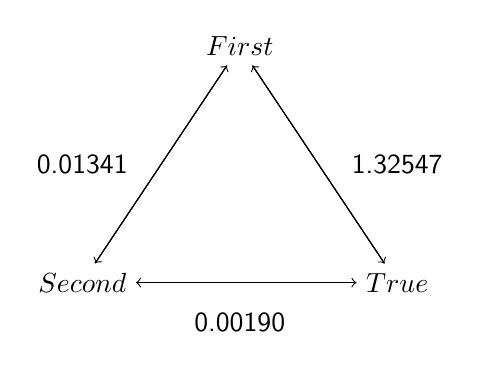
\begin{tikzpicture}
    \GraphInit[vstyle=Empty]
    %% Draw the nodes
    \node (A) at (5,3) {$First$};
    \node (B) at (3,0) {$Second$};
    \node (C) at (7,0) {$True$};
    %% Draw the alpha values
    \node (AB) at (3,1.5) {0.01341};
    \node (AC) at (7,1.5) {1.32547};
    \node (BC) at (5,-.5) {0.00190};
    %% Draw the edges
    \begin{scope}[every path/.style={->}]
      \draw (A) -- (B);
      \draw (B) -- (A);
      \draw (A) -- (C);
      \draw (C) -- (A);
      \draw (B) -- (C);
      \draw (C) -- (B);
    \end{scope}
  \end{tikzpicture}

  \vspace{1cm}
  Translated to confidence in paired difference: \\
  \vspace{0.5cm}

  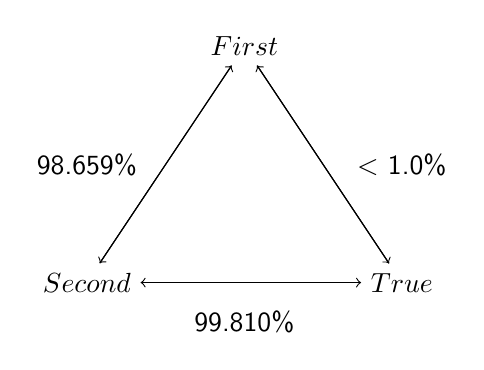
\begin{tikzpicture}
    \GraphInit[vstyle=Empty]
    %% Draw the nodes
    \node (A) at (5,3) {$First$};
    \node (B) at (3,0) {$Second$};
    \node (C) at (7,0) {$True$};
    %% Draw the alpha values
    \node (AB) at (3,1.5) {98.659\%};
    \node (AC) at (7,1.5) {\textless\ 1.0\%};
    \node (BC) at (5,-.5) {99.810\%};
    %% Draw the edges
    \begin{scope}[every path/.style={->}]
      \draw (A) -- (B);
      \draw (B) -- (A);
      \draw (A) -- (C);
      \draw (C) -- (A);
      \draw (B) -- (C);
      \draw (C) -- (B);
    \end{scope}
  \end{tikzpicture}
\end{center}

\vspace*{-3.5cm}
\hspace*{-3.5cm}
\includegraphics[page=7,width=27cm]{Raw-and-Fit-Report-Convergence-Over-100-Trials}
\captionof{figure}{In this CDF comparison, the \textit{second} CDF is
  once again the extreme outlier.}

\vspace*{-3.5cm}
\hspace*{-3.5cm}
\includegraphics[page=8,width=27cm]{Raw-and-Fit-Report-Convergence-Over-100-Trials}
\captionof{figure}{This KS Difference Plot follows similar trends to
  the previous 2.}

\vspace*{-3.5cm}
\hspace*{-3.5cm}
\includegraphics[page=9,width=27cm]{Raw-and-Fit-Report-Convergence-Over-100-Trials}
\captionof{figure}{This Confidence in KS Difference plot follows
  similar trends to the previous 2.}


\end{document}

%% pdflatex Report.tex && evince Report.pdf
